\documentclass[12pt, aspectratio=169]{beamer}

\usepackage{smu_beamer_template}
\usepackage{hyperref}
\usepackage{booktabs}
\usepackage{array}
\usepackage{colortbl}
\hypersetup{hidelinks}
\usepackage{verbatim}
\usepackage{listings}
\usepackage{amsmath, amssymb, amsthm}


\title[SMU Beamer Template]{A Simple \LaTeX{} Beamer Template for Southern Methodist University (SMU)}
\subtitle{with SMU-styled Color Themes and Fonts}
\author[Andrew Qing He]{Andrew Ho (Qing He)}
\institute[SMU Dept. Math]{Southern Methodist University, Department of Mathematics}
\date{\today}

\titletop{
{\centering
\includegraphics[height=0.12\textheight]{template-source/overleaf-logo-primary.png}\par}
}
\extrainfo{Email: andrewho@smu.edu\\{\color{SMUSalmon}\textit{This template is intended for non-commercial use only.}}}

% \color{SMUSalmon}For Overleaf users, please download this page, and set the main document to \texttt{main.tex} in the upper left \raisebox{-0.2\height}{
\includegraphics[height=1.5em]{template-source/overleaf_menu.png}}

\begin{document}

% Title slide
\begin{frame}[plain]
\titlepage
\end{frame}

% Table of contents
\begin{frame}{Outline}
\tableofcontents
\end{frame}

% ====================================
% SECTION: INTRODUCTION
% ====================================


\section{Introduction}

\begin{frame}{\insertsection}
\tableofcontents[currentsection]
\end{frame}

\begin{frame}{\insertsection}

This template provides a simple {\serif\LaTeX{}} Beamer design that follows Southern Me\-tho\-dist University's visual identity, as specified in the official brand guidelines at \href{https://www.smu.edu/brand}{\texttt{smu.edu/brand}}.

Due to its reliance on the \texttt{fontspec} package, this template requires compilation with \textbf{XeLaTeX}—it will not work with pdfLaTeX or LuaTeX.

Before you begin:
\begin{itemize}
    \item \textbf{\color{SMUSalmon}Save these slides} for future reference
    \item \textbf{\color{SMUSalmon}Set \texttt{main.tex} as your main document} in the Overleaf upperleft \raisebox{-0.2\height}{
\includegraphics[height=1.5em]{template-source/overleaf_menu.png}} 
\end{itemize}
if using this template on \raisebox{-0.1\height}{
\includegraphics[height=1.2em]{template-source/overleaf-logo-primary.png}}.
\end{frame}


\section{SMU Appearance Features}

\begin{frame}{\insertsection}
\tableofcontents[currentsection]
\end{frame}

\begin{frame}{\insertsection}

The core SMU style is built upon three key elements:
\begin{itemize}
    \item \raisebox{-0.15\height}{
\includegraphics[height=0.7\baselineskip]{template-source/SMU Logo_Formal_K.eps}} logo,
    \item \textbf{{\textcolor{SMUBlue}{S}}{\textcolor{SMURed}{M}}{\textcolor{SMUYellow}{U}}} color theme,
    \item {\serif\textbf{S}\textit{M}U} font set.
\end{itemize}
Together, these components form the university's signature aesthetic.
\end{frame}

\subsection{SMU Logos}
\begin{frame}{\insertsubsection}
    All logos in this template are sourced directly from the official SMU Box repository, linked from the university's brand site at \href{https://www.smu.edu/brand/logos}{\texttt{smu.edu/brand/logos}}.
    \vspace{8pt}
    \begin{columns}
        \begin{column}{0.2\textwidth}
        \centering
        
\includegraphics[width=.75\textwidth]{template-source/SMU_DallasHall_Icon_outlined_CMYK_lightbg.eps}
        \end{column}
        \begin{column}{0.2\textwidth}
        \centering
        
\includegraphics[width=.67\textwidth]{template-source/SMU Logo_Formal_K.eps}\vspace{4pt}        
        
\includegraphics[width=.67\textwidth]{template-source/SMU Logo_Formal_PMS_R.eps}\vspace{4pt}        
        
\includegraphics[width=.67\textwidth]{template-source/SMU Logo_Formal_PMS_B.eps}
        \end{column}
        \begin{column}{0.4\textwidth}
        % \centering
        
\includegraphics[height=0.077\textheight]{template-source/Lyle_FormalHrz_PMS_BR.eps}\vspace{4pt}
        
\includegraphics[height=0.07\textheight]{template-source/DedmanCollegeofHumanities&Sciences_FormalHrz_PMS_BR.eps}\vspace{4pt}
        
\includegraphics[height=0.07\textheight]{template-source/Moody_FormalHrz_PMS_BR.eps}    
        \end{column}
    \end{columns}
    \vspace{8pt}
    
    The official repository is available at:\\
    \centering\href{https://smu.app.box.com/s/bkdanzfumpcle67rfcqlakx3c9aa0lay}{\texttt{smu.app.box.com/s/bkdanzfumpcle67rfcqlakx3c9aa0lay}}
    
    \raggedright
    You can download any required logos directly from this source.
\end{frame}

\begin{frame}[fragile]{\insertsubsection}
Corrently, the Dallas Hall icon\ \raisebox{-0.35\height}{
\includegraphics[height=2\baselineskip]{template-source/SMU_DallasHall_Icon_outlined_CMYK_lightbg.eps}}\ is placed at the title page, and the department logo \ \raisebox{-0.25\height}{
\includegraphics[height=\baselineskip]{template-source/DedmanCollegeofHumanities&Sciences_FormalHrz_PMS_BR.eps}}\ is put at the lower right corner of each page with high transparency. Of course, these settings are all open to changes.
\begin{itemize}
    \item to change the title page logo (or do other background settings), find \verb|\titlegraphic{...}| command in the template file (\verb|smu_beamer_template.sty|), and replace the file name "\verb|...|" with your own logo file name.
    \item to change or remove the logo at the corner of each page, find \verb|\setbeamertemplate{background}{...}| code block in the template file, and modify the image file name in the \verb|\includegraphics| command.
\end{itemize}
\end{frame}

\subsection{SMU Color Theme}

\begin{frame}{\insertsubsection}
Unlike most universities and colleges in the world, SMU uses a series of high-saturation, high-contrast colors as the theme color of the university's brand. 
\begin{itemize}
    \item The \textcolor{SMUBlue}{\bf Blue} and \textcolor{SMURed}{\bf Red} colors are the primary colors
    \item \textcolor{SMUYellow}{\bf Yellow}, \textcolor{SMUSalmon}{\bf Salmon}, \textcolor{SMUTeal}{\bf Teal} and \textcolor{SMUBlack}{\bf Black} are secondary.
\end{itemize}
The details are listed below (source: \href{https://www.smu.edu/brand/color-palette}{\texttt{smu.edu/brand/color-palette}})
\begin{center}
\usetikzlibrary{positioning}
\begin{tikzpicture}[
    font=\sffamily\small,
    color box/.style={
        minimum width=2cm,
        minimum height=1.9cm,
        draw=black!20,
        line width=0.3pt,
        align=center,
        text width=1.8cm
    }
]

% Title
% \node[font=\large\bfseries] at (5, 3.3) {SMU Brand Color Palette};

% PRIMARY COLORS Section
\node[font=\small\bfseries, anchor=west] at (0, 2.6) {Primary Colors};

% SMU Blue
\node[color box, fill=SMUBlue, text=white, font=\tiny] at (1.2, 1.1) {
    \textbf{\normalsize Blue}\\[0.2cm]
    RGB: 53/76/161\\[0.05cm]
    \texttt{\#354CA1}\\[0.05cm]
    PMS 286
};

% SMU Red
\node[color box, fill=SMURed, text=white, font=\tiny] at (3.4, 1.1) {
    \textbf{\normalsize Red}\\[0.2cm]
    RGB: 204/0/53\\[0.05cm]
    \texttt{\#CC0035}\\[0.05cm]
    PMS 186
};

% SECONDARY COLORS Section
\node[font=\small\bfseries, anchor=west] at (5.4, 2.6) {Secondary Colors};

% Yellow
\node[color box, fill=SMUYellow, text=SMUBlack, font=\tiny, minimum width=1.6cm, minimum height=1.9cm, text width=1.4cm] at (6.4, 1.1) {
    \textbf{\scriptsize Yellow}\\[0.1cm]
    RGB:\\249/200/14\\[0.02cm]
    \texttt{\#F9C80E}\\[0.02cm]
    PMS 7548
};

% Salmon
\node[color box, fill=SMUSalmon, text=white, font=\tiny, minimum width=1.6cm, minimum height=1.9cm, text width=1.4cm] at (8.2, 1.1) {
    \textbf{\scriptsize Salmon}\\[0.1cm]
    RGB:\\255/16/83\\[0.02cm]
    \texttt{\#FF1053}\\[0.02cm]
    PMS 192
};

% Teal
\node[color box, fill=SMUTeal, text=SMUBlack, font=\tiny, minimum width=1.6cm, minimum height=1.9cm, text width=1.4cm] at (10, 1.1) {
    \textbf{\scriptsize Teal}\\[0.1cm]
    RGB:\\89/195/195\\[0.02cm]
    \texttt{\#59C3C3}\\[0.02cm]
    PMS 325
};

% Black
\node[color box, fill=SMUBlack, text=white, font=\tiny, minimum width=1.6cm, minimum height=1.9cm, text width=1.4cm] at (11.8, 1.1) {
    \textbf{\scriptsize Black}\\[0.1cm]
    RGB:\\38/38/38\\[0.02cm]
    \texttt{\#262626}\\[0.02cm]
    PMS 426
};

% Vertical separator line
\draw[gray, thick] (5.0, 0.1) -- (5.0, 2.8);

% Footer note
% \node[font=\small, text=black] at (6, -0.35) {};

\end{tikzpicture}
\end{center}
\end{frame}

\begin{frame}[fragile]{\insertsubsection}
These colors are defined as \textcolor{SMUBlue}{\texttt{SMUBlue}}, \textcolor{SMURed}{\texttt{SMURed}}, \textcolor{SMUYellow}{\texttt{SMUYellow}}, \textcolor{SMUSalmon}{\texttt{SMUSalmon}}, \textcolor{SMUTeal}{\texttt{SMUTeal}} and \textcolor{SMUBlack}{\texttt{SMUBlack}} through the \texttt{xcolor} package, so you may use them in the conventional way. For example, the commands
\vspace{-0.5em}
\begin{itemize}
    \item \lstinline[basicstyle=\ttfamily\small]|Please \textcolor{SMUBlue}{water} the \textcolor{SMURed}{flower}.|
    \item \lstinline[basicstyle=\ttfamily\small]|Please {\color{SMUBlue}water} the {\color{SMURed}flower}.|
\end{itemize}
\vspace{-0.5em}
both compiles to
{\par\centering
Please {\color{SMUBlue}water} the {\color{SMURed}flower}.
\par}
The latter can also be used in math formula. For example,
{\par\centering 
\verb|$$\frac{x^2}{2} {\color{SMUSalmon} + C}$$| \ \ compiles to\ \  $\displaystyle \frac{x^2}{2}{\color{SMUSalmon} + C}$.
\par}

% In practice, the frequencies of these colors have the order
% {\par\centering
% \textcolor{SMUBlue}{\bf Blue} > \textcolor{SMURed}{\bf Red} > \textcolor{SMUYellow}{\bf Yellow} > \textcolor{SMUSalmon}{\bf Salmon}\&\textcolor{SMUTeal}{\bf Teal}
% \par}
\end{frame}

\begin{frame}[fragile]{\insertsubsection}
Besides the text, we also use SMU color themes for the theorem blocks:
\begin{block}{Block Title}
You can use \verb|\begin{block}{Block Title} ... \end{block}| to generate a default block like this, whose default color is set as SMU Blue.
\end{block}
\begin{alertblock}{Alert Title}
You can use \verb|\begin{block}{Alert Title} ... \end{block}| to generate an alert block like this, whose default color is set as SMU Red.
\end{alertblock}
\begin{exampleblock}{Example Title}
You can use \verb|\begin{block}{Example Title} ... \end{block}| to generate an example block like this, whose default color is set as SMU Yellow.
\end{exampleblock}
\end{frame}

\begin{frame}[fragile]{\insertsubsection}
One who wants to change the color of these boxes may look for the following commands and modify the color in "\verb|{...}|") to the desired ones.
\begin{itemize}
    \item \verb|\setbeamercolor{block title}{...}|,\\ \verb|\setbeamercolor{block body}{...}|
    \item \verb|\setbeamercolor{block title alerted}{...}|,\\ \verb|\setbeamercolor{block body alerted}{...}|
    \item \verb|\setbeamercolor{block title example}{...}|,\\ \verb|\setbeamercolor{block body example}{...}|
\end{itemize}
When using SMU's colors, keep this order of importance in mind:
{\par\centering
\textcolor{SMUBlue}{\bf Blue} $>$ \textcolor{SMURed}{\bf Red} $>$ \textcolor{SMUYellow}{\bf Yellow} $>$ \textcolor{SMUSalmon}{\bf Salmon} $\approx$ \textcolor{SMUTeal}{\bf Teal},
\par}
Use this as a helpful guide when choosing which colors to feature in your slides.
\end{frame}

\begin{frame}[fragile]{\insertsubsection}
\textcolor{SMUSalmon}{Salmon} and \textcolor{SMUTeal}{Teal} are almost never used in formal occasions at SMU. Therefore, we did not set them as default colors for any element in this template. 

Nevertheless, they're more vibrant and eye-catching than \textcolor{SMURed}{Red} and \textcolor{SMUBlue}{Blue}, so you may use them for emphasis, usually together with bolding (\verb|\textbf| or \verb|\bf|)
\begin{itemize}
    \item Use \textcolor{SMUSalmon}{Salmon} to highlight one concept:
    \begin{itemize}
        \item It is the \textcolor{SMUSalmon}{\bf hydrogen bond} that combines the two DNA strands.
        \item Gradient descent usually converges to a \textcolor{SMUSalmon}{\bf local} minimum.
    \end{itemize}
    
    \item Use \textcolor{SMUSalmon}{Salmon} and \textcolor{SMUTeal}{Teal} to contrast two concepts:
    \begin{itemize}
        \item For a flow with a high Reynolds number, we are more likely to observe a \textcolor{SMUSalmon}{\bf turbulent flow} than a \textcolor{SMUTeal!85!black}{\bf laminar flow}.
    \end{itemize}
\end{itemize}
({\color{SMUTeal}Teal} is too shallow, so we used \verb|\color{SMUTeal!85!black}| in the last example to make it darker. Here \texttt{85} means "85\% Teal+15\% black).
\end{frame}

\subsection{SMU Fonts}

\begin{frame}{\insertsubsection}
\centering
{\huge \bf \serif The Font Makes a Difference!}\\
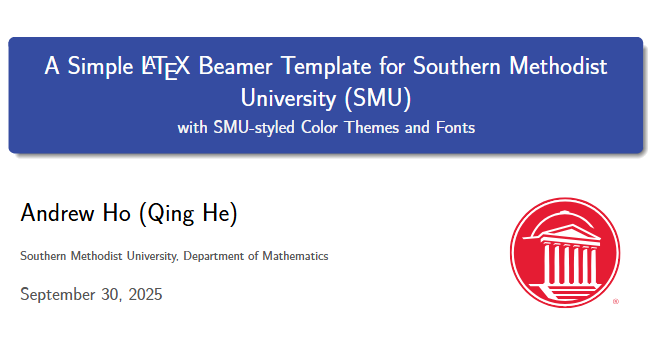
\includegraphics[height=0.45\textheight]{template-source/template_without_font.png}
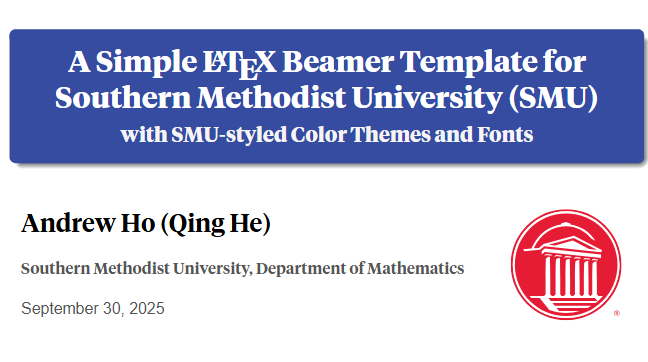
\includegraphics[height=0.45\textheight]{template-source/template_with_font.png}\\
\textbf{Even with identical logos and colors, \\different fonts create completely different impressions.}
\end{frame}

\begin{frame}{\insertsubsection}
\begin{columns}
    \begin{column}{0.6\textwidth}
        According to \href{https://www.smu.edu/brand/fonts}{\texttt{smu.edu/brand/fonts}}, SMU’s official brand fonts are
        \begin{itemize}
            \item Serif: Tiempos,
            \item Sans Serif: Trade Gothic,
        \end{itemize}
        and acceptable alternatives are Georgia (serif) and Arial (sans serif). 
        \vskip0.5em\par
        Although declairing "Both fonts can be used for headlines and/or body copy", SMU uses \textbf{\color{SMUSalmon}\serif serif for Title} and \textbf{\color{SMUTeal}sans serif for body} most of the time, and the body is usually \textbf{\color{SMUTeal}not} in Trade Gothic.
        \vskip0.5em\par
        \textbf{We will follow this practice.}
    \end{column}
    \begin{column}{0.4\textwidth}
        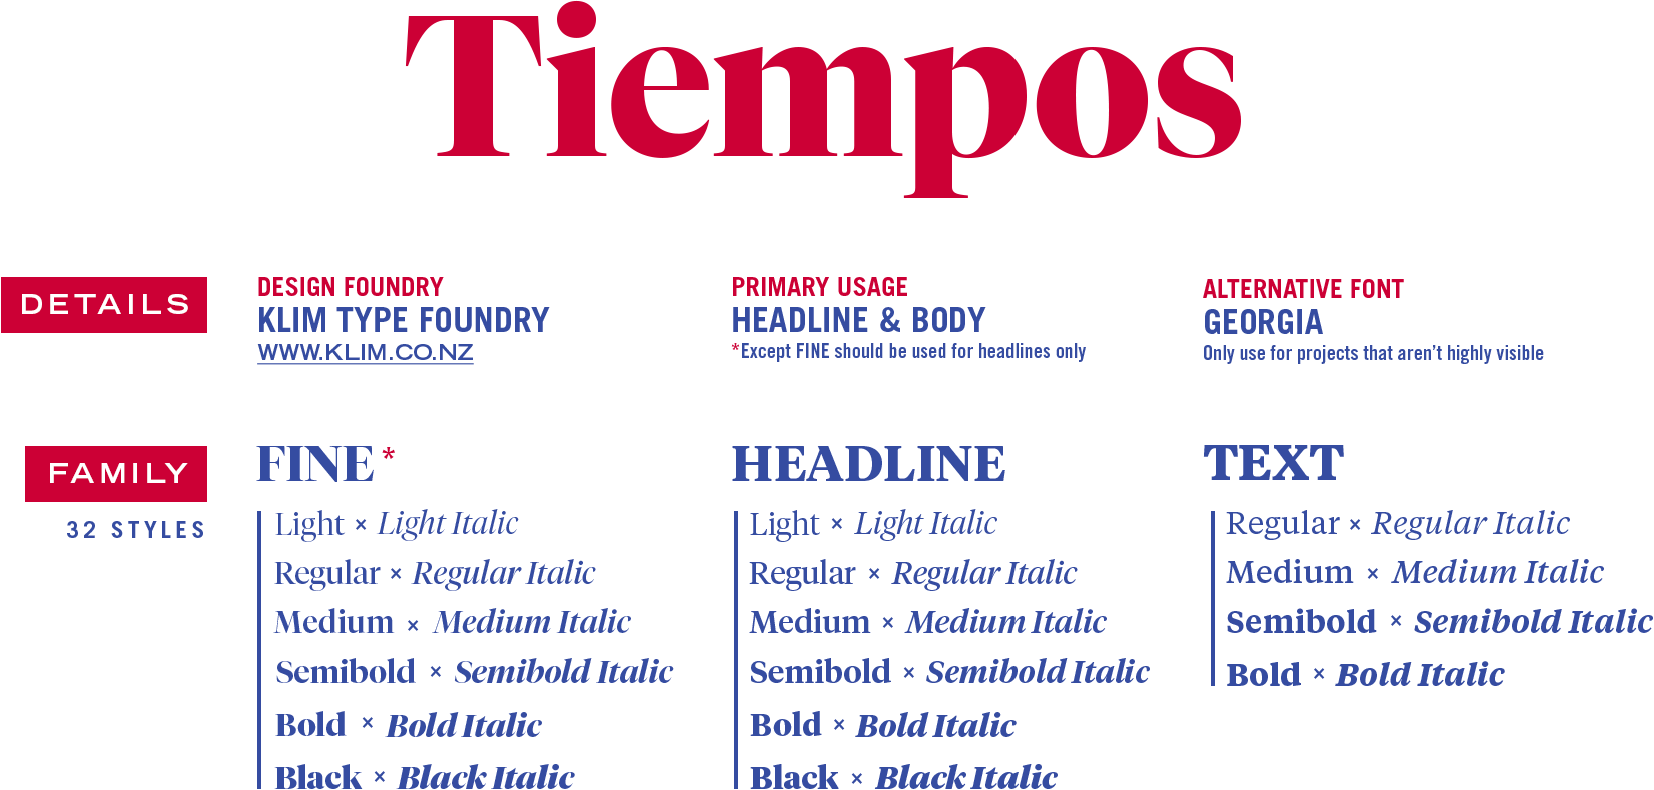
\includegraphics[width=\textwidth]{template-source/font_tiempos.png}
        \vskip2em\par
        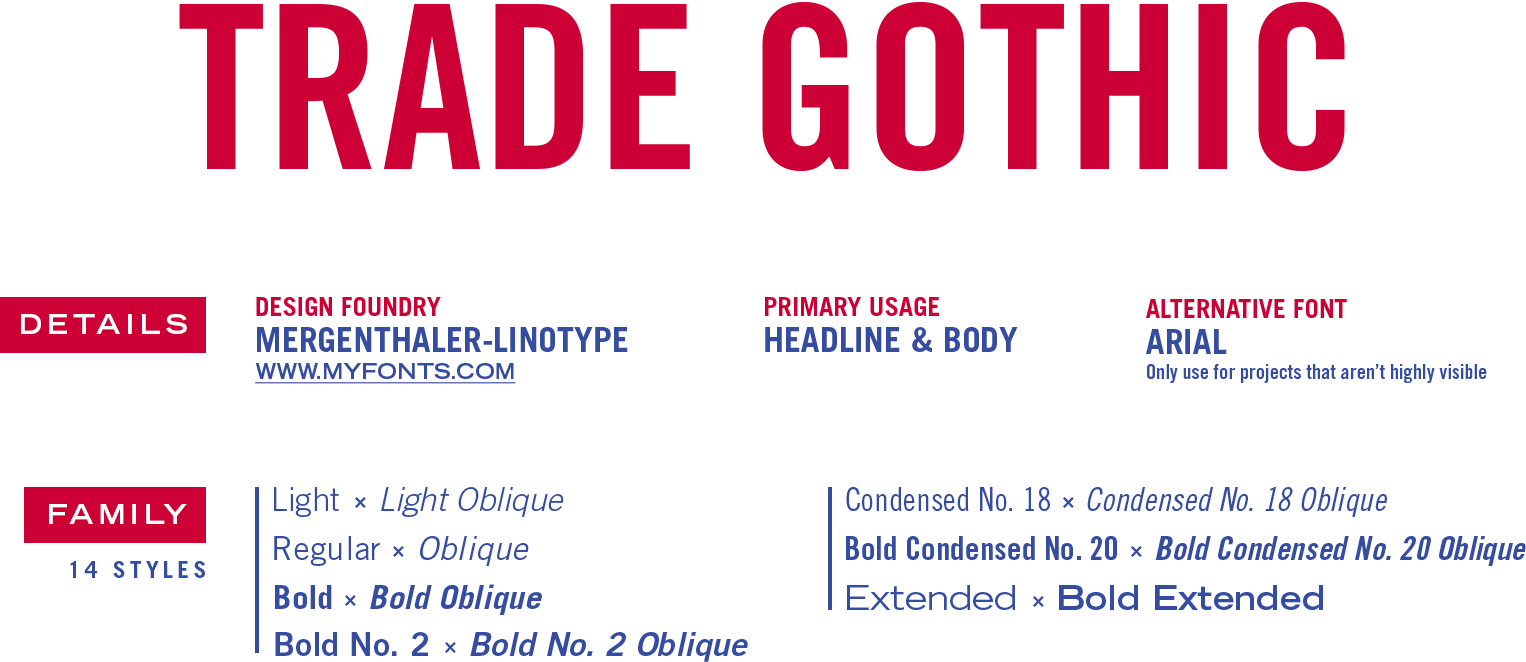
\includegraphics[width=\textwidth]{template-source/font_trade_gothic.png}
    \end{column}
\end{columns}
\end{frame}

\begin{frame}{\insertsubsection \ (Frame Title In Serif)}{Frame Subtitle in Serif}
This template uses {\serif\textbf{Tiempos Headline}} as the serif font, and \textbf{Arial} as the sans serif font. And following SMU's practice, we
\vskip-0.4em\par
\begin{itemize}
    \item use serif font only for the titles, subtitles and special cases (e.g. the big "{\fontseries{head}\serif THANK YOU}" at the end of the presentation).
    \begin{itemize}
        \item {\fontseries{head}\serif Fully Bold} for the {\fontseries{head}\serif Presentation Title and Subtitle},
        \item {\bf\serif Semibold} (default \texttt{\textbackslash{}textbf} font) for the {\bf\serif Frame Titles and Subtitles}.
        \item {\serif Regular serif font} is rarely used, included here only for completeness.
        \item Each of {\fontseries{head}\serif \textit{bold}}, {\bf\serif \textit{Semibold}}, {\it\serif Regular} has its Italic version.
    \end{itemize}
    \item use sans serif font for the contents (except formula and codes), including 
    \begin{itemize}
        \item normal text, listed items, tables
        \item title and content in a block (theorem, remark, example, etc.)
        \item captions of images, diagrams and tables.
        \item table of contents ... 
    \end{itemize}
\end{itemize}
\end{frame}

\begin{frame}[fragile]{\insertsubsection}
The \verb|\serif| command can be used for inputting serif contents e.g.
{\par\centering
\verb|{\serif\textbf{Southern} \textit{Methodist} University}|\par}
compiles to 
{\par\centering{\serif\textbf{Southern} \textit{Methodist} University.}\par}
Nevertheless, serif font is not encouraged to be used in the content unless for very special purposes.
\end{frame}

\begin{frame}[fragile]{Alternatives for Tiempos}
The font {\serif Tiempos} is commercial (we are using the test version of it). To avoid licensing issues, this template provides the free alternative \textbf{Source Serif 4}, available from \href{https://fonts.google.com/specimen/Source+Serif+4}{\color{SMUBlue}Google Fonts}.

We've included this font in \texttt{template-source/SourceSerif4}. To use it:
\begin{enumerate}
    \item Find and uncomment this block in the template (the \texttt{.sty} file): \verb|\newfontfamily\sourceserif[...]{SourceSerif4}|
    \item Also in the \texttt{.sty} file, find and change the command {\par\centering\verb|\def\serif{\tiempos}|\ \ into\ \ \verb|\def\serif{\sourceserif}|.\par}
\end{enumerate}
Of course, if you have your own preferred serif font (e.g. Georgia), you may also upload it and define it as the \verb|\serif| font. But this requires you to know how to use the \verb|\newfontfamily| command.
\end{frame}


\section{Other Features}
\begin{frame}{\insertsection}
    \tableofcontents[currentsection]
\end{frame}

\subsection{Math and Coding Fonts}

\begin{frame}[fragile]{The Math Formula Font}
In this template, we \textbf{\color{SMUSalmon}use the default math serif font in {\serif\LaTeX} for formula}, i.e.
{\par\centering
\verb|$x^2 + y^2$| compiles to $x^2 + y^2$ instead of \textit{x}\textsuperscript{2}$+$\textit{y}\textsuperscript{2}
\par}
One who wants the sans serif math formula may go to find the command
{\par\centering
\verb|\usefonttheme{professionalfonts}|
\par}
and remove it in the template file.
\begin{alertblock}{}\justifying
Beamer adopts a modern concept that sans serif fonts are more visually comfortable because of its simpleness, so it sets the default font for all elements as sans serif fonts, including mathematical formulas. However, in mathematics (and also many other disciplines), different fonts of notations make a big difference, and an arbitrary modification on the font is not a good practice.
\end{alertblock}

\end{frame}

\begin{frame}[fragile]{The Coding (Monospace) Font}
This template provides \textbf{JetBrains Mono} as the default monospace (\verb|\texttt|) font, which is the default coding font in JetBrains IDEs like PyCharm and IntelliJ. Its regular, bold and italic variations are as follows
\begin{itemize}
    \item \texttt{I am a Robot.}
    \item \textbf{\texttt{I am a heavy Robot.}}
    \item \textit{\texttt{I am a walking Robot.}}
    \item \textit{\textbf{\texttt{I am a heavy walking Robot.}}}
\end{itemize}
To adjust the \verb|\texttt| font, find and modify the \verb|\setmonofont{...}[...]| command in the template file \verb|smu_beamer_template.sty|.
\end{frame}

\begin{frame}[fragile]{The Coding (Monospace) Font}
Besides, the template supports syntax highlighting for multiple languages including C/C++, Java, Python, LaTeX, MATLAB, and Fortran. For example, to display Python code:
\begin{lstlisting}[style=python]
def hello_world():
    print("Hello, World!")
\end{lstlisting}
\vskip-0.5em
Wrap your code in the environment:
{\vskip-0.2em\par\centering
    \verb|\begin{lstlisting}[style=python] ... \end{lstlisting}|
\vskip-0.2em\par}
environment. 

You can modify existing styles or add new languages in \texttt{codestyle.tex} in the template-source directory.
\end{frame}

\subsection{Background Color and Frame Title}
\begin{frame}[fragile]{\insertsubsection}
The template provides two choices for the background (colored or white), and two choices for the header background (light or dark), so there are $2\times 2=4$ different combinations in total, from which you can pick the one you like.
\begin{itemize}
    \item See the next page for the visual result of the four combinations
\end{itemize}
To switch between these combinations, find the commands \verb|\usecolorbgtrue| and  \verb|\uselightheadertrue| in the template file.
\begin{itemize}
    \item Change \verb|\usecolorbgtrue| to \verb|\usecolorbgfalse| to use white background,
    \item Change \verb|\uselightheadertrue| to \verb|\uselightheaderfalse| use the header with dark background color.
\end{itemize}
\end{frame}


\begin{frame}
\begin{columns}
\begin{column}{0.5\textwidth}
\setbeamercolor{background}{}
    \centering
    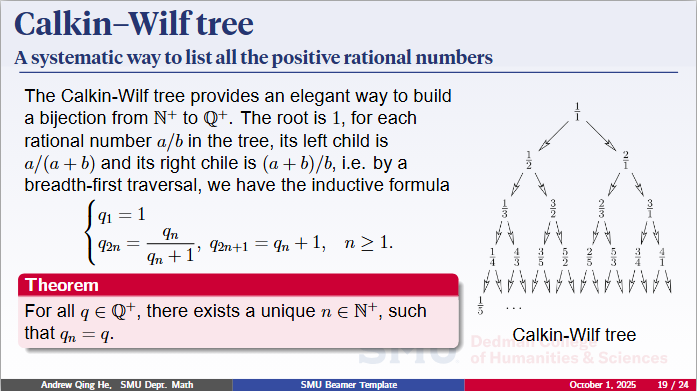
\includegraphics[width=0.8\textwidth]{template-source/sample_page_tt.png}
    
    colored background + light title
    \vskip0.5em\par
    
    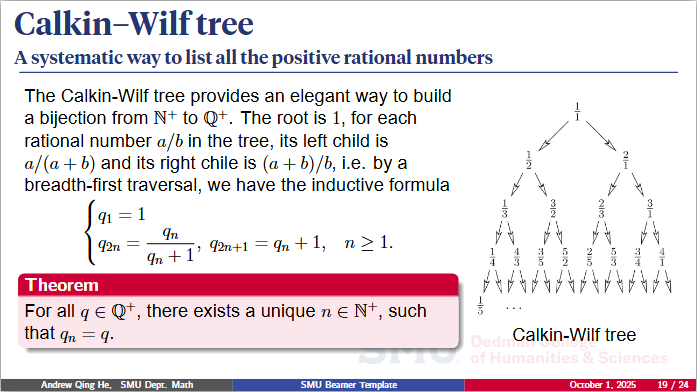
\includegraphics[width=0.8\textwidth]{template-source/sample_page_tf.png}
    
    white background + light title
    
\end{column}
\begin{column}{0.5\textwidth}
    \centering
    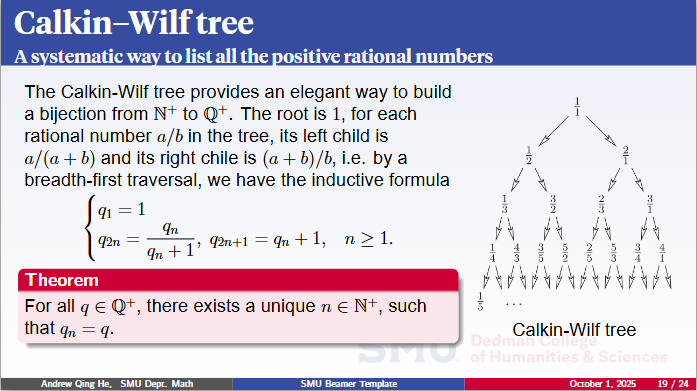
\includegraphics[width=0.8\textwidth]{template-source/sample_page_ft.png}

    colored background + dark title
    \vskip0.5em\par
    
    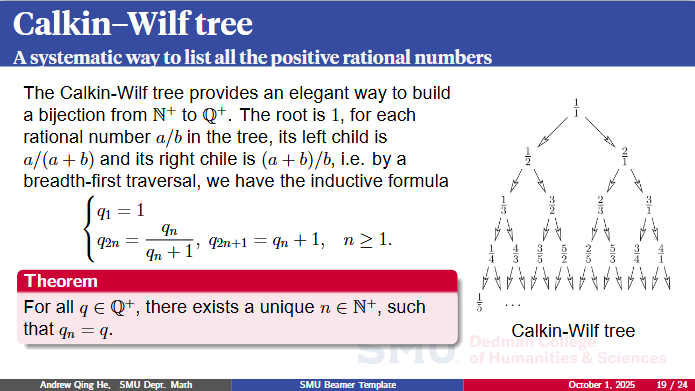
\includegraphics[width=0.8\textwidth]{template-source/sample_page_ff.png}
    
    white background + dark title
\end{column}
\end{columns}
\end{frame}

\subsection{Title Page}
\begin{frame}[fragile]{\insertsubsection}{}
\begin{columns}
    \begin{column}{0.5\textwidth}\justifying
        This template offers a flexible framework for designing your title page.
        \begin{itemize}\justifying
            \item \textbf{Above the title}: you can add conference logos, funder acknowledgments, or other organizational logos using \verb|\titletop{...}| in the header of \texttt{main.tex}.
            \item \textbf{Below your name and institute}: you can include additional information like collaborators, email addresses, or other details using \verb|\extrainfo{...}| in the header of \texttt{main.tex}.
        \end{itemize}
        
    \end{column}
    \begin{column}{0.49\textwidth}
        \begin{center}
        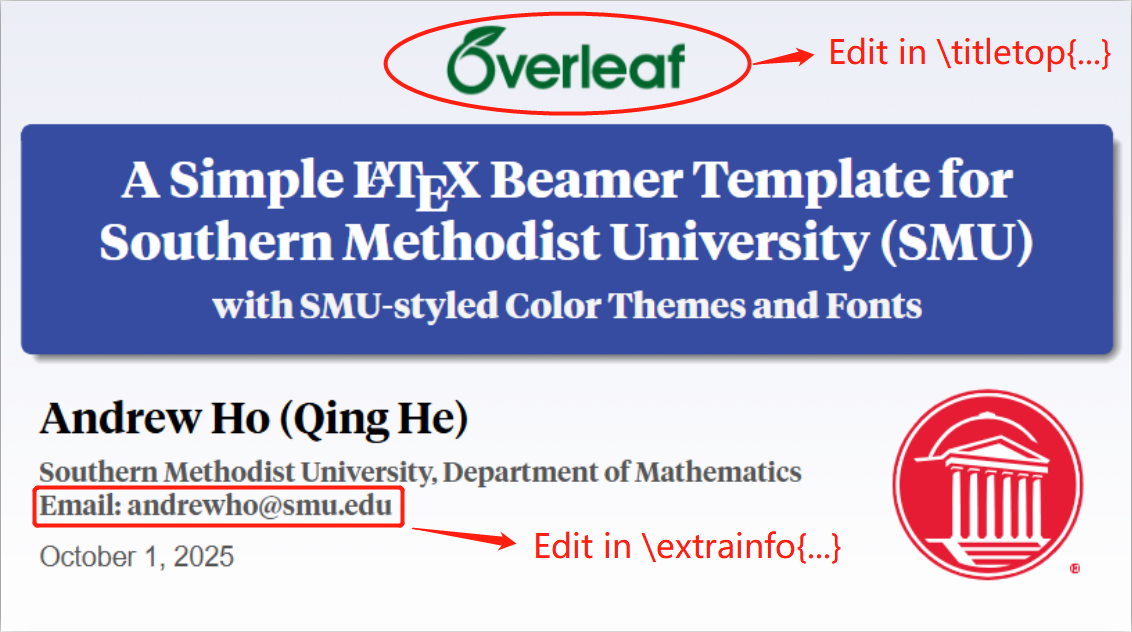
\includegraphics[width=\textwidth]{template-source/Template_title_editting.png}
        \begin{alertblock}{}
            \small \justifying You can add custom text and images in these two areas, but note that sizing, fonts, and alignment must be manually adjusted (e.g., centering logos yourself).
        \end{alertblock}
    \end{center}
    \end{column}
\end{columns}

\end{frame}

\section{Examples}
\begin{frame}{\insertsection}
    \tableofcontents[currentsection]
\end{frame}

\begin{frame}{Calkin–Wilf Tree}{A systematic way to list all the positive rational numbers}
\begin{columns}
    \begin{column}{0.65\textwidth}\justifying
        The Calkin-Wilf tree provides an elegant way to build a bijection from $\mathbb{N}^+$ to $\mathbb{Q}^+$. The root is $1$, for each rational number $a/b$ in the tree, its left child is $a/(a+b)$ and its right chile is $(a+b)/ b$, i.e. by a breadth-first traversal, we have the inductive formula
        \vskip-.8em\par$$
        \begin{cases}
            q_1 = 1 \\
            \displaystyle q_{2n} = \frac{q_n}{q_n+1},\ q_{2n+1}=q_n+1, & n \geq1.
        \end{cases}        
        $$\vskip-.8em\par
        \begin{alertblock}{Theorem}
          For all $q \in \mathbb{Q^+}$, there exists a unique $n \in \mathbb{N}^+$, such that $q_n = q$. 
        \end{alertblock}
    \end{column}
    \begin{column}{0.3\textwidth}
    \centering
    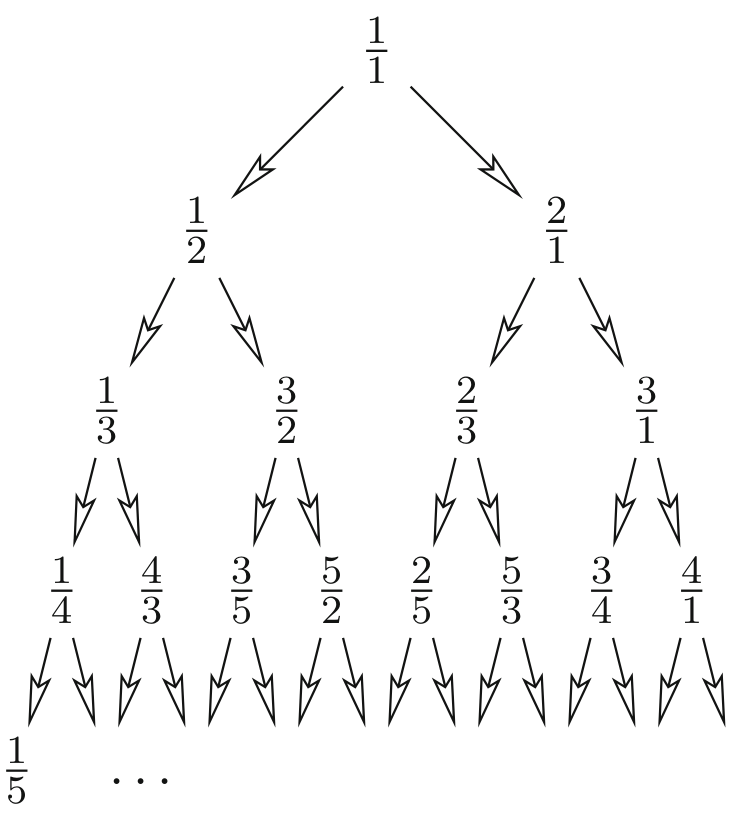
\includegraphics[width=\textwidth]{template-source/CWTree.png}\\
    Calkin-Wilf tree
    \end{column}
\end{columns}
\end{frame}

\begin{frame}{Comparison of the Complexity and Stability of Common Sorting Algorithms}{I wrote this long title and subtitle intentionally to show the template's ability to handle multiline titles. In reality, titles should be clear and neat}
\begin{table}[htbp]
\centering
% \caption{Detailed Comparison of Sorting Algorithms}
\label{tab:sorting_detailed}
\small
\begin{tabular}{@{}lccccc@{}}
\toprule
\textbf{Algorithm} & \textbf{Time (Avg)} & \textbf{Time (Worst)} & \textbf{Space} & \textbf{Stable} & \textbf{In-place} \\
\midrule
Bubble Sort & $O(n^2)$ & $O(n^2)$ & $O(1)$ & Yes & Yes \\
Selection Sort & $O(n^2)$ & $O(n^2)$ & $O(1)$ & No & Yes \\
Insertion Sort & $O(n^2)$ & $O(n^2)$ & $O(1)$ & Yes & Yes \\
Merge Sort & $O(n \log n)$ & $O(n \log n)$ & $O(n)$ & Yes & No \\
Quick Sort & $O(n \log n)$ & $O(n^2)$ & $O(\log n)$ & No & Yes \\
Heap Sort & $O(n \log n)$ & $O(n \log n)$ & $O(1)$ & No & Yes \\
Counting Sort & $O(n+k)$ & $O(n+k)$ & $O(k)$ & Yes & No \\
Radix Sort & $O(nk)$ & $O(nk)$ & $O(n+k)$ & Yes & No \\
Bucket Sort & $O(n+k)$ & $O(n^2)$ & $O(n)$ & Yes & No \\
% Tim Sort & $O(n \log n)$ & $O(n \log n)$ & $O(n)$ & Yes & No \\
\bottomrule
\end{tabular}
\end{table}
\end{frame}

\begin{frame}{Figures: Remove the Background Color}
When the background is not pure white, a good practice is to remove the background color before including any figures. This can leave a very good impression to your audience. 
\begin{figure}
    \centering
    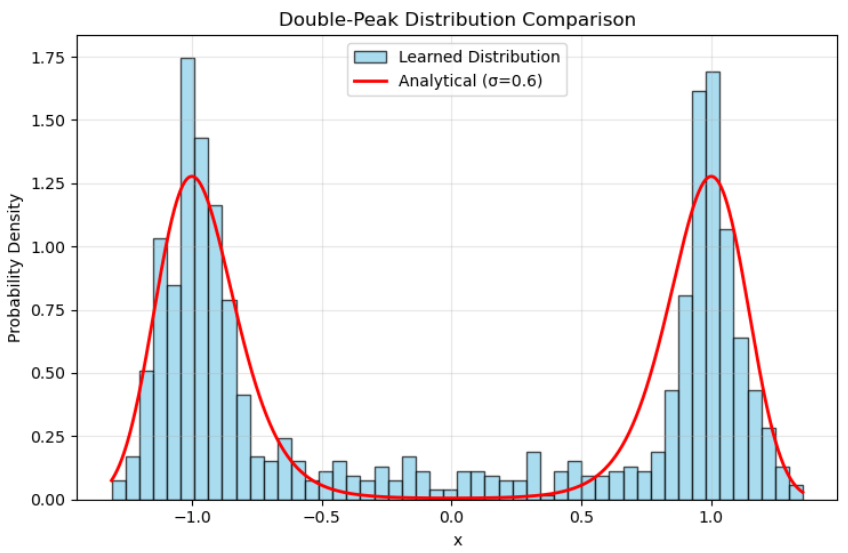
\includegraphics[width=0.4\linewidth]{template-source/double_peak_fig.png}\hspace{0.05\linewidth}
    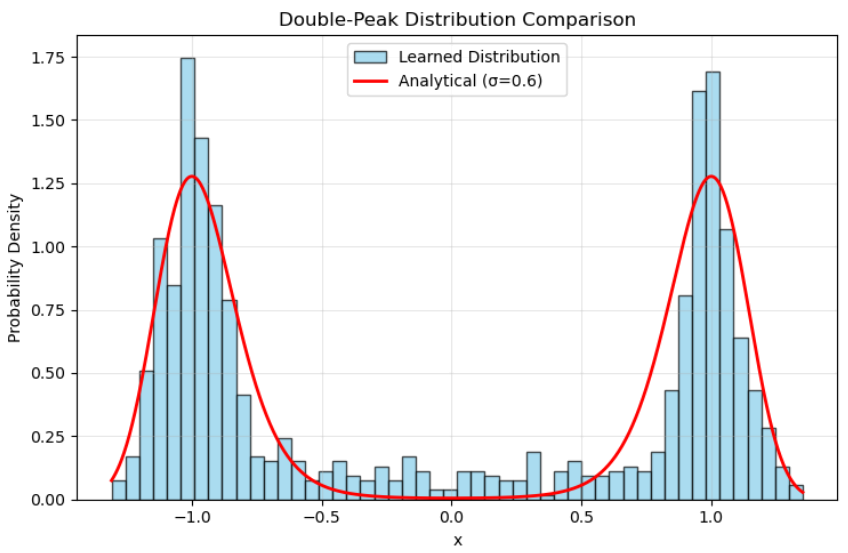
\includegraphics[width=0.4\linewidth]{template-source/double_peak_fig_rmbg.png}
    \caption{A figure before and after background removal}
    \label{fig:doublepeakbd}
\end{figure}
\end{frame}

\begin{frame}[fragile]{Figures: Remove the Background Color}
\begin{columns}
\begin{column}{0.65\linewidth}
\begin{lstlisting}[style=python]
from PIL import Image
def make_transparent(input_path, output_path):
    img = Image.open(input_path)
    if img.mode != 'RGBA':
        img = img.convert('RGBA')
    data = img.getdata()
    new_data = []
    for item in data:
        if min(item[:3]) > 250:
            new_data.append((255, 255, 255, 0))
        else:
            new_data.append(item)
    img.putdata(new_data)
    img.save(output_path, "PNG")
\end{lstlisting}
\end{column}
\begin{column}{0.3\linewidth}\justifying
A simple python script that reads an image from \verb|input_path|, sets the pixels with all the RGB value greater than 250 to transparent, and saves the background-removed version of the image to \verb|output_path|.
\end{column}
\end{columns}

\end{frame}



\begin{frame}[allowframebreaks]{References (Fake, Genereated by AI)}
\bibliographystyle{plain}  % or: alpha, ieeetr, apalike, abbrv
\nocite{*}
\bibliography{template-source/fake_references}
\end{frame}



{\setbeamertemplate{background}{}
\begin{frame}
\begin{tikzpicture}[remember picture, overlay]
    % Image layer (between bg color and text)
    \node[at=(current page.center), opacity=0.15, inner sep=0pt] {
        
\includegraphics[width=0.7\paperwidth]{template-source/Peruna_PMS_R.eps}
    };
\end{tikzpicture}

% The frame background color is still there
% Your text appears on top
\centering
{\serif\fontseries{head}\fontsize{40}{48}\selectfont\color{SMUBlue!95!black} THANK YOU!}
\vskip11pt\par
{\Huge \bf \serif\color{SMUBlue!95!black}Questions and Discussion}

{Notice that in this page, we have removed the logo at the corner. \\This is set by surrounding the frame with \\ \texttt{\{\textbackslash{}setbeamertemplate\{background\}\{\} ... \}}} \\
\end{frame}}

\end{document}